%=============================================================================
\documentclass[10pt,a4paper]{article}
%
\input{dd4hep-setup.tex}
%
\pagestyle{fancyplain}{\fancyfoot[C]{\sffamily{DDRec User Manual}}}
%
\usepackage{amsmath}
\begin{document}   
%
\mytitle{
DDRec
}{
Reconstruction Interface for the \\
\vspace{0.5cm}
dd4hep Geometry Description \\
\vspace{0.5cm}
Toolkit
\vspace{2cm}
}{
%M.Frank%\textsuperscript{1},
F.Gaede%\textsuperscript{2},
%C.Grefe\textsuperscript{1},
%P.Mato\textsuperscript{1}

%{\textsuperscript{1} 
{CERN, 1211 Geneva 23, Switzerland}

%{\textsuperscript{2} 
{Desy, 22607 Hamburg, Germany}
}
%
%
%==  Abstract  ===============================================================
\pagestyle{plain}
\pagenumbering{Roman}
\setcounter{page}{1}
\begin{abstract}
%=============================================================================

\noindent
\normalsize
The reconstruction of particle tracks and clusters in an High Energy Physics detector
requires information about the geometrical and material properties of the various 
tracking and calorimeter subdetectors.
In general, a higher level view on the detector geometry is needed than for the purpose
of simulating the detailed detector response with tools such as Geant4\cite{bib:geant4}.
This higher level view typically involves the abstraction of detector layers, the corresponding
measurement surfaces, accumulation of dead material along a path and conversion between cellIDs and 
positions.
While in principle it is of course possible to extract this information from the detailed 
detector geometry model used for simulation, doing so would tightly couple the reconstruction
code to the specific implementation of the simulation model. 
\DDR provides a generalized API for reconstruction that can be used to decouple the details of 
the \DDH\cite{bib:dd4hep} detector geometry model from the reconstruction algorithms.
 
\end{abstract}

\vspace{8cm}

\begin{center}
{\large{\bf{
\begin{tabular} {| l | l | l |}
\hline
\multicolumn{3}{| c |}{} \\[0.2cm]
\multicolumn{3}{| c |}{Document History} \\[0.2cm]
\multicolumn{3}{| c |}{} \\[0.2cm]
\hline
                 &      &        \\
Document         &      &        \\
version          & Date & Author \\[0.2cm] \hline
                 &      &        \\
1.0              & 11/11/2014 & Frank Gaede CERN/DESY  \\
                 &      &        \\        \hline 
\end{tabular}
}}}
\end{center}

\clearpage
%
%
%==  TOC  ====================================================================
\tableofcontents
\clearpage
%
%
%=============================================================================
% Manual
%=============================================================================
\pagenumbering{arabic}
\setcounter{page}{1}

%=============================================================================
\section{Introduction}
\label{sec:ddrec-manual-introduction}
%=============================================================================
\noindent
This manual introduces the \DDR package which is part of \DDH and provides the 
high level view on the HEP detector geometry that is needed during reconstruction and 
analysis. 
In the detailed simulation of the response of a typical High Energy Physics detector
very little information is needed in principle on the actual structure of the material
distribution in the detector. This becomes obvious if one considers the fact that
the Geant4 program is also used in medical applications where the human body 
is approximated by a voxelised phantom.
During the reconstruction of particle trajectories and calorimeter clusters, in particular 
in the phase of pattern recognition, one typically regards the detector as an abstract
structure of measurement surfaces or volumes that generally follow a layering structure.
\DDR contains an API that provides this information for reconstruction algorithms, thereby
decoupling the details of the actual simulation model used from the reconstruction code.
\noindent
The \DDR API provides the following functionality:

\begin{itemize}\itemcompact
\item description of measurement surfaces with coordinate systems for 
  track finding and fitting
\item description of non-active surfaces with material properties in
  order to take effects of multiple scattering and energy loss
  into account
\item conversion of cellIDs assigned to simulated tracker and calorimeter hits
  to positions of readout cells and vice versa
\item access to a list of materials between any two points inside the world
  volume of the detector
\item access to the materials at any given point or along a straight line between two points
\item averaged material properties for a list of materials
\item computation of radiation and interaction lengths for detector layers, modules
  or arbitrary sections through the detector
\end{itemize}

\noindent
In this manual we describe the different classes in \DDR and how they should be
used in the detector geometry constructors as well as in the reconstruction
code. 

\subsection*{Doxygen code documentation}
Please also refer to the code documentation that is created with doxygen for more
details on the classes and their members. This documentation can be build with:

\begin{unnumberedcode} 
   cmake -D INSTALL_DOC=ON ${path_to_dd4hep_source}
   make install
\end{unnumberedcode}

\noindent
and will then be available at
\begin{unnumberedcode} 
   ${DD4hepINSTALL}/doc/html/index.html
\end{unnumberedcode}

%=============================================================================
\section{Surfaces}
\label{sec:ddrec-manual-surfaces}
%=============================================================================
For fitting the trajectories of charged particle tracks one generally needs to know 
the measurement surfaces on which the hits where deposited. Additionally the material 
properties along the trajectory need to be known in order to correct for effects
from multiple scattering and energy loss. 
\DDR provides an abstract interface for surfaces and materials in the namespace
{\em DDSurfaces} and a concrete implementation, described below, in the namespace
{\em DDRec}. This is done in order to separate interface and implementation and allow
other software tools, e.g. tracking packages to just use the interface.
 
%=============================================================================
\subsection{namespace DDSurfaces}
\label{subsec:ddrec-ddsurfaces}
%=============================================================================
The basic concept of surfaces in \DDR is expressed with the two main interfaces
{\em ISurface} and {\em IMaterial}. They are shown together with helper classes in
the {\em DDSurfaces} in figure:\ref{fig:ddrec_ddsurfaces_classes}
and are briefly described in the following.

\begin{figure}[h]
  \begin{center}
    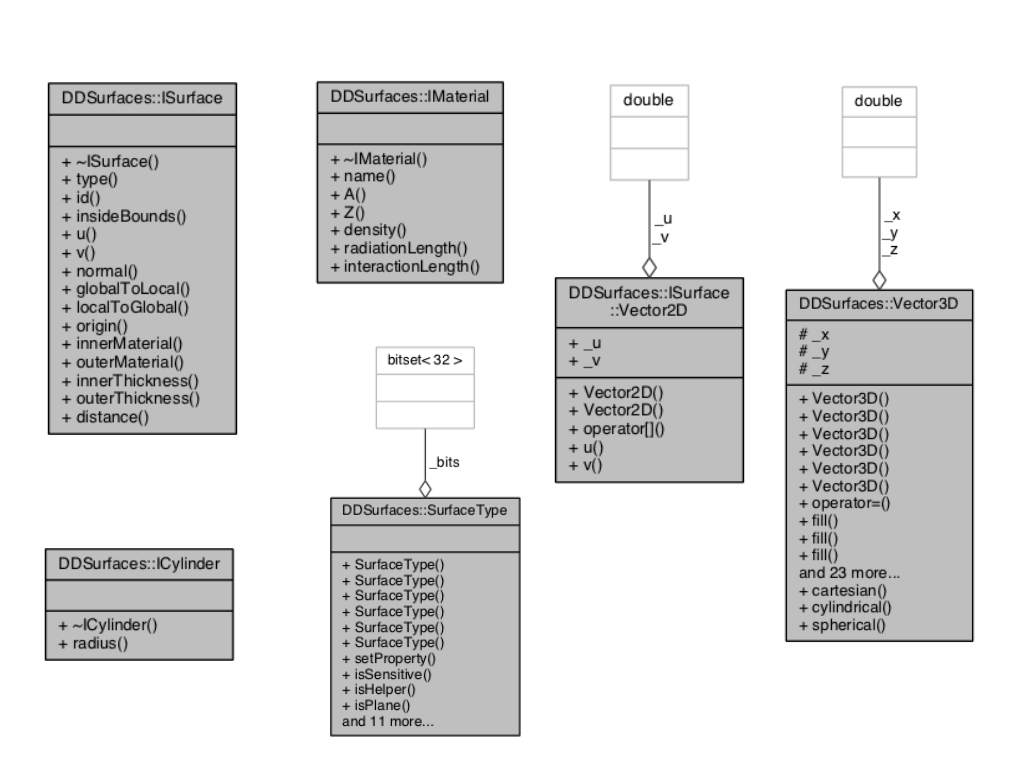
\includegraphics[width=120mm] {DDRec_ISurface_classes.png}
    \caption{Classes in namespace DDSurfaces: abstract interfaces {\em ISurface, IMaterial, ICylinder}
      and helper classes {\em Vector3D, ISurface::Vector2D, SurfaceType}. }
    \label{fig:ddrec_ddsurfaces_classes}
  \end{center}
\end{figure}

\noindent{\em \bf ISurface}: Defines the surface by means of an origin, a normal vector n and two, 
typically orthogonal, direction vectors u and v, where all of the vectors n,u,v might depend 
on the actual position on (or close to) the surface. In order to describe material properties
two thicknesses are assigned to the surface - one in direction of the normal vector (outerThickness) 
and one in the opposite direction (innerThickness). There are two materials assigned to these
thicknesses, where these materials could be averaged along the normal and thickness.
The method {\em isInsideBounds} allows in principle to implement arbitrary bounds for the surface.
Two methods allow the conversion between global 3d coordinates (on the surface) and local 2d coordinates 
in the coordinate system of the surface.
 
\noindent
{\em \bf IMaterial}: Interface to describe the relevant material properties: atomic number and weight, 
density and radiation- and interaction lengths. These can be real materials or averaged materials along
a given direction and length (thickness assigned to the surface).

\noindent
{\em \bf ICylinder}: Simple interface for cylindrical surfaces adding the cyliner radius to a surface
through multiple inheritance.

\noindent
{\em \bf ISurface::Vector2D} Helper struct inside ISurface for 2d vectors with coordinates u and v.

\noindent
{\em \bf Vector3D}: Generic 3d vector class with cartesian coordinates x,y,z that allows initialization
from other 3d vector implementations or using cylindircal or spherical coordinates. Provides acces to
quantities often needed, such as magnitude, transversal component, representation in non-cartesian
coordinates.

\noindent
{\em \bf SurfaceType}: Helper class using an {\em std::bitfield<32>} to encode the 
following properties of the surface: {\em isCylinder, isPlane, isSensitive, isHelper} (dead material),
{\em isParallelToZ, isOrthogonalToZ, isInvisible, isMeasurement1D}.

%=============================================================================
\subsection{Surface implementation}
\label{subsec:ddrec-ddsurfaces}
%=============================================================================
\DDR provides classes that implement the interface defined in {\em DDSurfaces}.
The main classes for implementing {\em ISurface} are shown in 
figure \ref{fig:ddrec_surfaces_classes}.

\begin{figure}[h]
  \begin{center}
    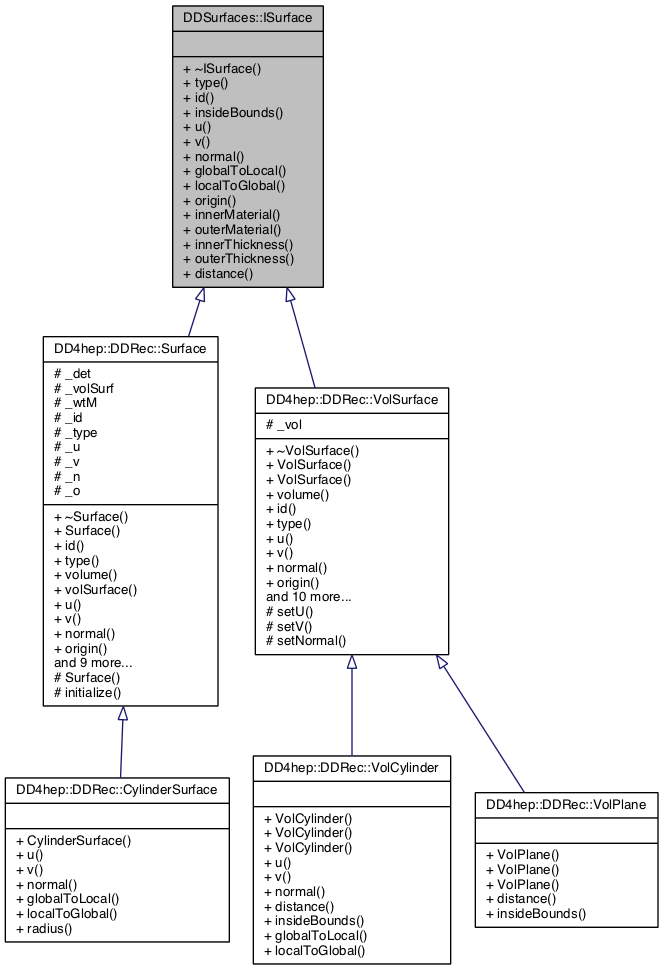
\includegraphics[width=100mm] {DDRec_surface_classes.png}
    \caption{Class diagram with the main classes describing detector
      surfaces and their relations.}
    \label{fig:ddrec_surfaces_classes}
  \end{center}
\end{figure}

\noindent
The implementation of the surfaces in \DDR is done in two parallel hierarchies 
of implementation classes. The first hierarchy is based on the {\em VolSurface}
class which connects a surface with its surrounding volume.
This volume then provide the boundaries of the surface and gives access to 
the local to global coordinate transformations inside the coordinate system
of the volume. There are currently two concrete implementations: 
{\em VolCylinder} and {\em VolPlane} that can be used in the detector construction
code as described in\ref{subsec:ddrec-surfaces-constructors}.
The second hierarchy is the actual implementation of the surface concept in \DDR
to be used by reconstruction code as described in \ref{subsec:ddrec-surfaces-reconstruction}.
It uses the extension and views concept described in the main \DDH manual\cite{bib:dd4hepManual}.
The {\em Surface} class has a {\em VolSurface} object and a {\em DetElement} and 
uses these to establish the local to global coordinate transforms, the surface boundaries
and the material properties. The materials on both sides of the surface are
the averaged materials along the direction of the normal with the given thicknesses.
It is thus possible to also take material effects into account for materials
that lay outside of the actual volume the surface is attached to.
This is in particular useful for compound materials that consist of a larger number
of thin slices.

%=============================================================================
\subsection{Using surfaces in geometry constructors}
\label{subsec:ddrec-surfaces-constructors}
%=============================================================================
The surfaces that should be available in the reconstruction code, 
have to be assigned to their corresponding volume and detector element by the 
user in the detector geometry construction code. 
This is done by specifying the coordinate system
and orientation of the surface inside the volume with vectors o,n,u and v 
and then instantiating one of the two types {\em VolCylinder} or {\em VolPlane} for a 
given volume.
After the placement of the corresponding DetElement, the surface is added to the
list of surfaces for this DetElement.

\noindent
This is demonstrated in the  following example code:

\begin{code}
  #include "DDRec/Surface.h"
  //...
  // base vectors for surfaces:
  DDSurfaces::Vector3D o(0,0,0) ;
  DDSurfaces::Vector3D u(1,0,0) ;
  DDSurfaces::Vector3D v(0,1,0) ;
  DDSurfaces::Vector3D n(0,0,1) ;

  // --- loop over layers ----
  // ...

    dd4hep::Box  box( dimX/2, dimY/2, dimZ/2 ) ;
    dd4hep::Volume vol( volumeName, description.material( x_layer.materialStr() )) ;

    dd4hep::DetElement layerDetElement( parentDetElement , "layer"+_toString(i,"_%02d") , det_id ) ;

    // add a measurement surface to the layer for every sensitive slice:

    dd4hep::rec::VolPlane surf( vol , 
                          DDSurfaces::SurfaceType(DDSurfaces::SurfaceType::Sensitive),
                          dimZ, dimZ, 
                          u, v, n , o ) ; 

    // place the layer
    dd4hep::PlacedVolume pv = parentVol.placeVolume(  vol, layerPlacement );

    layerDetElement.setPlacement( pv ) ;

    dd4hep::rec::volSurfaceList( layerDetElement )->push_back( surf ) ;

  // --- end loop over layers ----

\end{code}
In this example a planar ({\em VolPlane}) measurement ({\em SurfaceType(Sensitive)})
surface is attached to the box volume of a detector layer.
The thickness of the surface corresponds to that of the box and is given by its half length in z
( Vector3D n(0,0,1) runs along z). Thus the surface is completely contained in 
the box and no averaging of materials will be done, unless additional volumes
are placed inside the box at a later stage. 
The origin of the coordinate system of the surface coinsides with that of the box
({\em Vector3D o(0,0,0); })
and the two measurememnt directions u,v run along the x and y axis of the box
respectively.

\noindent
The following code snipped shows the creation of a cylindrical surface attached
to a tube volume for the inner field cage of a tpc. The radius of the cylindrical
surface is given by the transversal component of the origin vector {\em ocyl}.
The volume {\em innerWallVol} is filled with air and will be later populated
with slices of a compound material, thus the material properties will be
averaged along the thickness of the tube.

\begin{code}
  //...
  dd4hep::Tube innerWallSolid(rInner ,rInner + dr_InnerWall ,dz_Wall / 2.0 ) ;

  dd4hep::Volume innerWallVol( "TPCInnerWallVol", innerWallSolid, materialAir ) ; 

  pv = tpc_motherLog.placeVolume( innerWallVol ) ;

  DDSurfaces::Vector3D ocyl(  rInner + 0.5*dr_InnerWall , 0. , 0. ) ;

  dd4hep::rec::VolCylinder surfI( innerWallVol , 
                                    SurfaceType( SurfaceType::Helper ) ,
                                    0.5*dr_InnerWall, 0.5*dr_InnerWall, 
                                    ocyl ) ;

  volSurfaceList( tpc )->push_back(  surfI ) ;
  //...
\end{code}




%=============================================================================
\subsection{Using surfaces in reconstruction code}
\label{subsec:ddrec-surfaces-reconstruction}
%=============================================================================
Accessing and using the surfaces in reconstruction code is very easy. 
There are two possibilities to access the surfaces:
\begin{itemize}
\item use the {\em DetectorSurfaces} view class to get a list of 
 all surfaces that have been assigned to a particular {\em DetElement}
 object.
\item or use the {\em SurfaceManager} class to get a list of all
 surfaces of a given {\em DetElement} and all its daughters.
\end{itemize}

\noindent
The following code snippet uses the {\em SurfaceManager}, initialized
with the world  {\em DetElement}, to get a list of all surfaces 
defined for a given detector model.
The surfaces are then printed to {\em std::cout} and filled 
into a map, using the surfaces ID as a key.
For sensitive surfaces, attached to sensitive volumes, the ID
will be that of the sensitve volume and thus such a map provides
a very easy lookup from the hitID to its corresponding measurement
surface.

\begin{code}
  // ...

  dd4hep::Detector& description = dd4hep::Detector::getInstance();

  description.fromCompact( inFile );

  dd4hep::DetElement world = description.world() ;

  // create a list of all surfaces in the detector:
  dd4hep::rec::SurfaceManager surfMan(  world ) ;

  const dd4hep::rec::SurfaceList& sL = surfMan.surfaceList() ;

  // map of surfaces
  std::map< long64, dd4hep::rec::Surface* > surfMap ;

  for( dd4hep::rec::SurfaceList::const_iterator it = sL.begin() ; it != sL.end() ; ++it ){
    
    dd4hep::rec::Surface* surf =  *it ;
    
    std::cout << " ------------------------- " 
      	      << " surface: "  << *surf         << std::endl
      	      << " ------------------------- "  << std::endl ;
    
    surfMap[ surf->id() ] = surf ;
  }

\end{code}

\noindent
And similarily this code uses the {\em DetectorSurfaces} class to just access the surfaces 
for a particular detector element:

\begin{code}
  // ...

  dd4hep::DetElement ladderDE = description.detector("VXD_layer02_ladder42") ;

  // create surfaces
  dd4hep::rec::DetectorSurfaces ds( ladderDE ) ;

  const dd4hep::rec::SurfaceList& detSL = ds.surfaceList() ;

  for( dd4hep::rec::SurfaceList::const_iterator it = detSL.begin() ; it != detSL.end() ; ++it ){

    dd4hep::rec::Surface* surf =  *it ;

    std::cout << " ------------------------- " 
      	      << " surface: "  << *surf         << std::endl
      	      << " ------------------------- "  << std::endl ;
  }
\end{code}

%=============================================================================
\subsection{Visualizing detector surfaces}
\label{subsec:ddrec-surfaces-visualization}
%=============================================================================

The detector surfaces and the vectors defining their coordinate system can be
visualized with the program {\em teveDisplay} that is part of \DDH. In a future
version of \DDH this visualization might be included in \DDE.
Currently a full 3d view of the detector surfaces as well as a $\rho-\phi$-view
and a $\rho$-z view are available. See figure~\ref{fig:ddrec_surfaces_visualization}.

\begin{figure}[h]
  \begin{center}
    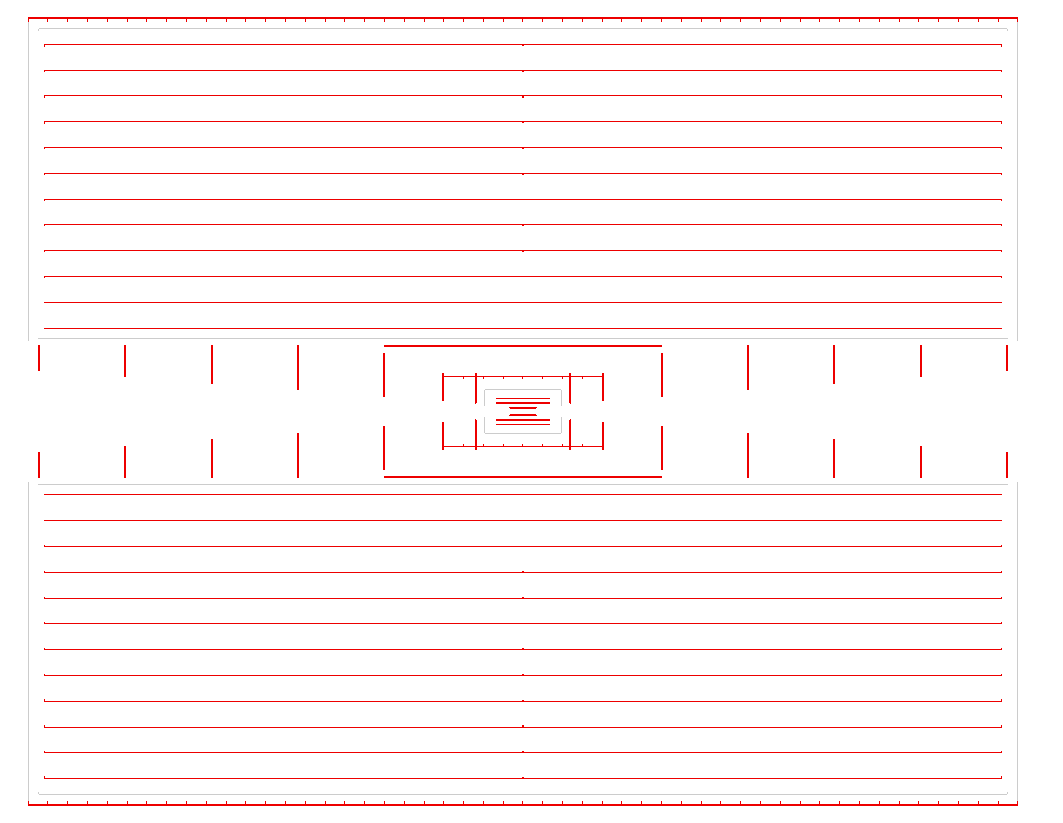
\includegraphics[width=0.48\hsize]{DDRec_rhoz_surfaces.png} 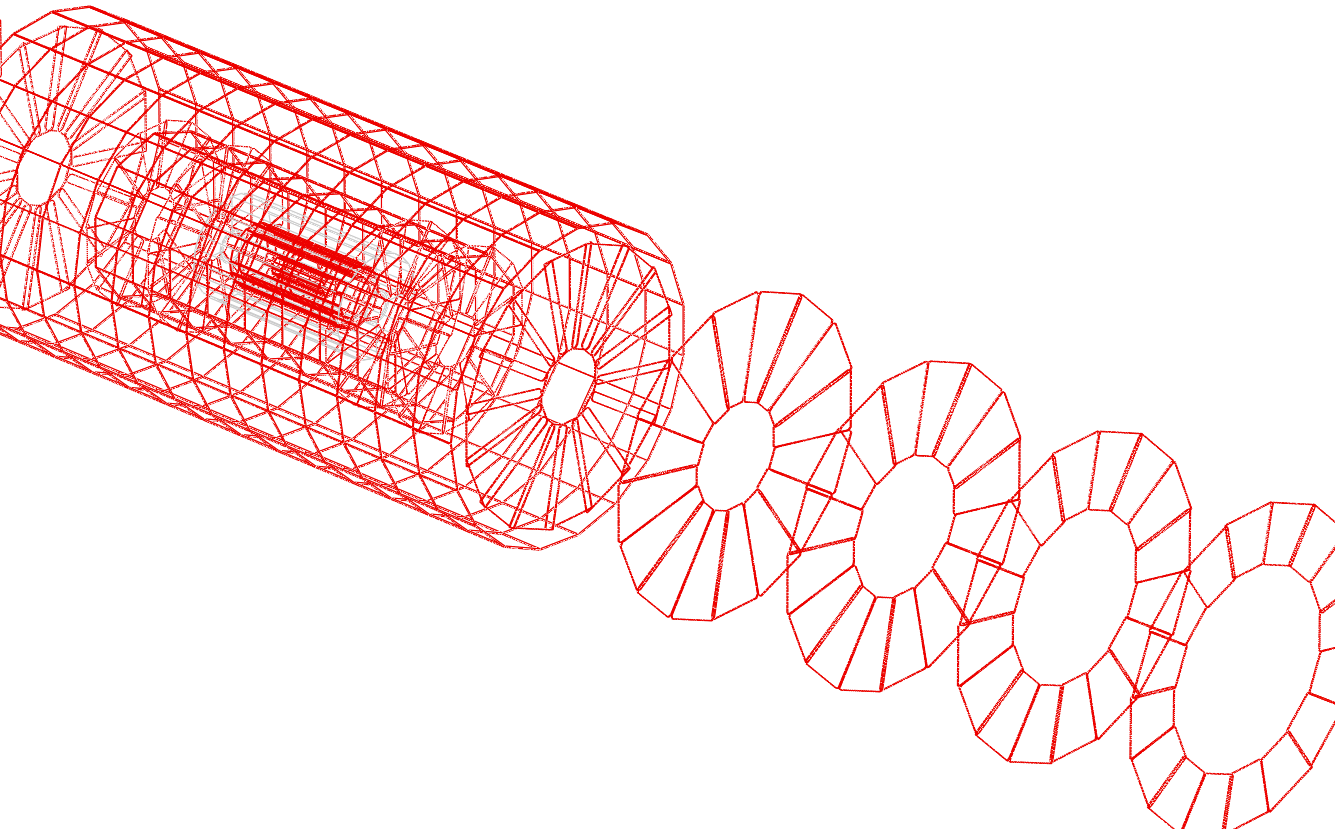
\includegraphics[width=0.48\hsize]{DDRec_inner_tracking_surfaces.png}
    \caption{Example of surface visualization. Left: $\rho$-z view of the tracking surfaces in the ILD detector, Right: 3D view of the 
    surfaces in the inner tracking detectors in ILD.}
    \label{fig:ddrec_surfaces_visualization}
  \end{center}
\end{figure}
 


%=============================================================================
\section{Materials}
\label{sec:ddrec-manual-materials}
%=============================================================================
The surfaces classes described above provide a way that allows to
augment a detector geometry description with a high level view on the detector
that should be sufficient for most reconstruction tasks, such as pattern
recognition, track fitting and calorimeter reconstruction as in a particle 
flow algorithm. However they require that care has been taken to assign all
relevant surfaces with corresponding thicknesses to the volumes and detector
elements. For cases where this is not possible or where other reconstruction
geometries should be instantiated, \DDR provides the possibility to access
the materials at any given point in the world volume of the detector or 
to retrieve a list of materials along a straight line between any two points.

\noindent
This is done with the class {\em MaterialManager}, which also allows to
create an averaged material for a list of materials ({\em MaterialVector}).
The usage of this class is simple and best demonstrated with an example:

\begin{code}

  dd4hep::Detector& description = dd4hep::Detector::getInstance();

  description.fromCompact( inFile );

  DDSurfaces::Vector3D p0( x0, y0, z0 ) ;
  DDSurfaces::Vector3D p1( x1, y1, z1 ) ;

  dd4hep::rec::MaterialManager matMgr ;

  const dd4hep::rec::MaterialVec& materials = matMgr.materialsBetween( p0 , p1  ) ;
	
  std::cout  << std::endl  
             << " #######  materials between the two  points : " 
             << p0 << "*cm  and " << p1 << "*cm :  "  
             << std::endl ;

  double sum_x0 = 0 ;
  double sum_lambda = 0 ;
  double path_length = 0 ;
  for( unsigned i=0,n=materials.size();i<n;++i){

    dd4hep::rec::Material mat =  materials[i].first  ;
    double length = materials[i].second  ;

    double nx0 = length / mat.radLength()  ;
    sum_x0 += nx0 ;

    double nLambda = length / mat.intLength()  ;
    sum_lambda += nLambda ;

    path_length += length ;

    std::cout << "      "               << mat 
              << " thickness: "         << length 
              << " path_length:"        << path_length
              << " integrated_X0: "     << sum_x0 
              << " integrated_lambda: " << sum_lambda 
              <<  std::endl ;
  }

\end{code}

\noindent
Creation of an averaged material:

\begin{code}
  // ...
  const dd4hep::rec::MaterialVec& materials = matMgr.materialsBetween( p0 , p1  ) ;
	
  const dd4hep::rec::MaterialData& avMat = matMgr.createAveragedMaterial( materials ) ;

  std::cout << " averaged Material : " << " Z: " << avMat.Z() << " A: " << avMat.A() 
            << " densitiy: "           << avMat.density()
            << " radiationLength: "    << avMat.radiationLength() 
            << " interactionLength: "  << avMat.interactionLength()  
            << std::endl ;
\end{code}

\noindent
There is a utility program {\em print\_materials} that can be used to debug detector
geometries:

\begin{verbatim}
 $ print_materials
 usage: print_materials compact.xml x0 y0 z0 x1 y1 z1
        -> prints the materials on a straight line between the two given points ( unit is cm)
\end{verbatim}


\noindent
{\bf Note: accessing the materials using the {\em MaterialManager} is a rather
costly operation and should only be done at the initialization phase 
of a reconstruction program for caching material properties !}



%=============================================================================
\section{IDDecoder}
\label{sec:ddrec-manual-iddecoder}
%=============================================================================
Sensitive volumes in a \DDH geometry model are assigned a unique volume-ID. 
This ID is then used by the corresponding {\em DDSegmentation} object
to create a unique cellID for tracker and calorimeter hits, allowing
to uniquely match hits to their sensitive volumes and also to their
{\em DetElements} if they have been defined appropriately.
During reconstruction tasks, including digitization of simulated hits,
one often needs to convert between a cellID assigned to the hit and 
the position of the corresponding detector cell. 
For example one could write out simulated calorimeter hits without position
information in order to save disk space and retrieve the position information
based on the cellID. Another application might be a clustering algorithm
where one looks for hits in the neighbor cells of a given hit.

\noindent
The functionality to do this is provided by the {\em IDDecoder} class with
the following interface:

\begin{code}
  class IDDecoder {
  public:
     /// Default constructor using the name of the corresponding readout collection
    IDDecoder(const std::string& collectionName);
    
     /// Default constructor using a readout object
    IDDecoder(const Readout& readout);
    
     /// Destructor
    virtual ~IDDecoder();
    
     /// Returns the cell ID from the local position in the given volume ID.
    CellID cellIDFromLocal(const Position& local, const VolumeID volumeID) const;
    
     /// Returns the global cell ID from a given global position
    CellID cellID(const Position& global) const;
    
     /// Returns the global position from a given cell ID
    Position position(const CellID& cellID) const;
    
     /// Returns the local position from a given cell ID
    Position localPosition(const CellID& cellID) const;
    
     /// Returns the volume ID of a given cell ID
    VolumeID volumeID(const CellID& cellID) const;
    
     /// Returns the volume ID of a given global position
    VolumeID volumeID(const Position& global) const;
    
     /// Returns the placement for a given cell ID
    PlacedVolume placement(const CellID& cellID) const;
    
     /// Returns the placement for a given global position
    PlacedVolume placement(const Position& global) const;
    
     /// Returns the subdetector for a given cell ID
    DetElement subDetector(const CellID& cellID) const;
    
     /// Returns the subdetector for a given global position
    DetElement subDetector(const Position& global) const;
    
     /// Returns the closest detector element in the hierarchy for a given cell ID
    DetElement detectorElement(const CellID& cellID) const;
    
     /// Returns the closest detector element in the hierarchy for a given global position
    DetElement detectorElement(const Position& global) const;
    
     /// Calculates the neighbours of the given cell ID and adds them to the list of neighbours
    void neighbours(const CellID& cellID, std::set<CellID>& neighbours) const;
    
     /// Checks if the given cell IDs are neighbours
    bool areNeighbours(const CellID& cellID, const CellID& otherCellID) const;
}
\end{code}




%=============================================================================
\section{Detectors}
\label{sec:ddrec-manual-detectors}
%=============================================================================
To be done ...



\newpage
%=============================================================================
\begin{thebibliography}{9}
\bibitem{bib:dd4hep} M. Frank et al, "dd4hep: A Detector Description Toolkit 
                for High Energy Physics Experiments",
                detailtional Conference on Computing in High Energy and Nuclear Physics  
                (CHEP 2013), \\
                Amsterdam, Netherlands, 2013, proceedings.
                
\bibitem{bib:dd4hepManual} M. Frank et al, "dd4hep: A Detector Description Toolkit 
                for High Energy Physics Experiments", Users manual (dd4hepManual.pdf).
                

\bibitem{bib:ROOT-tgeo} R.Brun, A.Gheata, M.Gheata, "The ROOT geometry package",\\
                    Nuclear Instruments and Methods {\bf{A}} 502 (2003) 676-680.

\bibitem{bib:geant4}  S. Agostinelli et al., 
                   "Geant4 - A Simulation Toolkit", \\
                    Nuclear Instruments and Methods {\bf{A}} 506 (2003) 250-303.

\end{thebibliography}
%=============================================================================
\end{document}
